\documentclass[../main.tex]{subfiles}

\begin{document}

\chapter{初步使用计算机}

我们已经讲过了计算机的基本构成和工作原理,现在我们来讲一些计算机的初步使用方法。

当然,我们不会涉及到计算机的使用细节,例如如何使用鼠标、如何使用键盘等。我们假设同学们已经具备了最基本的计算机操作能力。这里将会介绍一些科研学习中使用计算机的小技巧,以及一些常用的软件和工具。

\section{维护你的系统}

计算机的维护是一个非常重要的环节。我们需要定期对计算机进行清理和维护,以保证计算机的正常运行。

\subsection{保持更新系统的习惯}

计算机在运行过程中,操作系统和软件会不断地更新,以修复漏洞、提高性能和增加新功能。我们应该定期检查系统和软件的更新,并及时按需要安装它们。

对于一些重要的更新(例如安全更新等),我们应该立即安装,这是因为此类更新通常是为了修复一些新近发现的漏洞和问题,如果不及时安装,可能会导致计算机被攻击或者出现其他问题。而对于一些不重要的更新(例如功能更新等),我们可以根据自己的需要选择安装。

特别注意:虽然我们提倡保持更新,但是在生产类环境中,贸然更新可能会导致系统不稳定或软件不兼容。因此,在生产环境中,我们应该在更新之前进行充分的测试,确保更新不会影响系统的正常运行,或者使用虚拟机等隔离环境运行生产用代码。

\subsection{定期备份数据}

定期备份数据是保护计算机数据安全的重要措施。我们可以使用外部硬盘、云存储等方式备份数据,以防止信息泄露或者重要文件丢失。数据备份的频率可以根据数据的重要性和变化频率来决定。

数据备份有一个重要的原则:\textbf{3-2-1备份法则}。即:至少保留三份数据备份,存储在两个不同的介质上,其中一份存储在异地。例如,我们可以在本地硬盘上存储一份数据备份,在外部硬盘上存储一份数据备份,并将另一份数据备份存储在云端。这样,即使其中一份甚至两份损坏或者丢失,我们也可以通过其他方式恢复数据。

\subsection{定期清理系统}

定期清理系统可以提高计算机的性能和安全性。我们可以使用一些系统清理工具,删除不必要的文件、缓存和临时文件等,以释放磁盘空间和提高系统性能。我们推荐使用系统自带的清理工具,例如Windows的磁盘清理工具、macOS的存储管理工具等。如果较为富裕,也可以使用一些知名的清理软件,例如CCleaner等(免费版已经足够好用了)。出于众所周知的原因,我们不推荐使用360等软件。

除此之外,休眠文件、系统还原点等也会占用大量磁盘空间。我们可以根据自己的需要,选择是否保留这些文件。

特别注意的是,清理系统和减肥差不多,同样需要\textbf{缓慢、谨慎、循序渐进}地进行。

\subsection{碎片整理}

在计算机使用过程中,如果使用机械硬盘,文件的删除和修改会导致磁盘上的数据变得零散,从而影响计算机的性能。我们可以使用碎片整理工具,定期对磁盘进行碎片整理(即重排文件使其连续),以部分提高磁盘的读写速度。

直接使用Windows自带的碎片整理工具即可。对于固态硬盘,碎片整理并不会提高性能,反而会缩短使用寿命,因此不建议对SSD进行碎片整理。

\section{善用快捷键}

使用快捷键可以减少鼠标操作的频率。以下是来自Windows的常用快捷键:

\begin{table}[htbp]
  \centering
  \caption{Windows常用快捷键}
  \label{tab:windows-shortcuts}
  \begin{tabular}[t]{c|c}
    \hline
    \textbf{快捷键} & \textbf{功能} \\
    \hline
    \texttt{Ctrl+C} & 复制 \\
    \texttt{Ctrl+V} & 粘贴 \\
    \texttt{Ctrl+Z} & 撤销 \\
    \texttt{Ctrl+Y} & 重做 \\
    \texttt{Ctrl+A} & 全选 \\
    \texttt{Ctrl+Alt+Del} & 打开任务管理器 \\
    \texttt{Ctrl+S} & 保存当前文档或文件 \\
    \texttt{Ctrl+P} & 打印当前文档或文件 \\
    \texttt{Ctrl+F} & 查找文本或内容 \\
    \hline
  \end{tabular}
  \qquad
  \begin{tabular}[t]{c|c}
    \hline
    \textbf{快捷键} & \textbf{功能} \\
    \hline
    \texttt{Alt+F4} & 关闭当前窗口 \\
    \texttt{Alt+Tab} & 迅速切换窗口 \\
    \texttt{Win+R} & 打开运行窗口 \\
    \texttt{Win+E} & 打开文件资源管理器 \\
    \texttt{Win+D} & 显示桌面 \\
    \texttt{Win+L} & 锁定计算机 \\
    \texttt{PrtScn} & 截图(全屏) \\
    \texttt{Alt+PrtScn} & 截图(当前窗口) \\
    \texttt{Win+Shift+S} & 截图(自定义区域) \\
    \hline
  \end{tabular}
\end{table}

除了上述快捷键以外,在其他的软件中也有着自己特定的快捷键。例如在浏览器中,Ctrl+T可以打开一个新的标签页,Ctrl+W可以关闭当前标签页,Ctrl+Shift+T可以重新打开上一个关闭的标签页等。这些快捷键可以帮助我们更高效地使用计算机。

\section{终端初步}\label{sec:terminal}

终端是计算机与操作系统之间的一个交互界面。它允许用户通过命令行输入指令,与操作系统进行交互。

虽然终端是一个非常古老的工具,但是使用它依然可以提高工作效率,尤其是在处理大量文件或者进行复杂操作时。它还可以用于远程连接到其他计算机,进行远程管理和维护等操作。

一般情况下,一条命令满足以下结构:
\begin{lstlisting}[language=bash]
    <命令> [<选项>] [<参数>]
\end{lstlisting}

其中,命令是要执行的操作,选项是对命令的补充说明(例如 -h 往往表示帮助信息),参数是命令的输入(例如文件名)。选项和参数往往都是可选的。

对于Linux和macOS,常见的shell有以下几种:

\begin{table}[ht]
  \centering
  \begin{tabular}{c|ccc}
    \hline
    & \textbf{bash} & \textbf{zsh} & \textbf{fish} \\
    \hline
    定位 & 通用,默认 & 高度定制 & 易用、美观、现代化 \\
    兼容性 & POSIX标准兼容 & 大多数兼容bash & 不兼容bash,自成一套 \\
    上手难度 & 中等 & 中等偏高 & 非常简单 \\
    自动补全 & 仅有基础功能 & 需配合插件 & 开箱即用 \\
    语法高亮 & 没有 & 有插件 & 默认有 \\
    可定制性 & 较低 & 非常高 & 较高 \\
    脚本通用性 & 几乎全通用 & 高 & 低 \\
    资源占用 & 非常低 & 取决于插件 & 较低 \\
    \hline 
  \end{tabular}
  \caption{常见的Linux/macOS Shell对比}
\end{table}
我们推荐使用zsh或者fish。关于zsh怎么安装插件的问题,可以参考网上的各种教程,例如Oh My Zsh等。

对于Windows,默认的终端是CMD,其风格太老了,基本与现代开发脱节,不建议使用。我们建议使用Windows PowerShell。PowerShell的命令统一采用的是动词-名词的格式,和Linux Shell的简单缩写形式有很大的不同。这是因为PowerShell的设计理念是模仿C\#的“对象”,而不是Linux Shell的文本流。不过也正因此,PowerShell本身就是一门完备的语言,功能非常强大,在处理复杂的任务上更为简单。

除了这些以外,如果不希望使用Windows的原生终端,也可以使用诸如Cygwin、MSYS2等类Unix环境,来获得类似Linux的终端体验。有些教程会让你使用git bash,这东西是一个精简版MSYS2,主要用于Git操作,功能非常有限,不建议长期使用。

下表\ref{tab:terminal-commands}是一些常见的命令。

\begin{table}[htbp]
  \centering
  \begin{tabular}{c|cc}
    \hline
    \textbf{操作} & \textbf{\*sh类系统} & \textbf{Pwsh} \\
    \hline
    创建文件 & touch & New-Item \\
    列出文件 & ls & Get-ChildItem \\
    复制文件 & cp & Copy-Item \\
    移动文件 & mv & Move-Item \\
    删除文件 & rm & Remove-Item \\
    创建目录 & mkdir & New-Item -Type Directory \\
    删除目录 & rmdir & Remove-Item -Recurse \\
    查看帮助 & man & Get-Help \\
    \hline
  \end{tabular}
  \caption{Bash和PowerShell的常用命令对比}
  \label{tab:terminal-commands}
\end{table}

这仅仅是最基本的命令使用方法,实际上终端的命令系统非常复杂,功能也非常强大。感兴趣的同学可以自行查找相关资料进一步学习。

\section{包管理器}

包管理器是用于管理软件包的工具。它可以自动下载、安装、升级和卸载软件包,并且可以解决软件包之间的依赖关系。

在Linux和macOS中,包管理器是非常常用的工具。它可以帮助用户快速安装和管理软件包,避免手动下载和安装软件包的麻烦。比如我希望在Arch Linux下安装GCC,只需要执行以下命令即可:

\begin{lstlisting}[language=bash]
    sudo pacman -S gcc
\end{lstlisting}

在Windows中,包管理器的使用不普遍。虽然有一个官方的包管理器winget,但是支持的软件包较少,且无法自动管理依赖(但也基本够用);还有一些例如Chocolatey、Scoop等第三方包管理器。除此以外,使用MSYS2、Cygwin等类Unix环境也可以从某种程度上当成包管理器使用。例如后文讲的安装GCC的过程,我们就是使用MSYS2来安装的,比下载预编译版本简单许多。

\section{Git初步}\label{sec:git}

试想以下环境:我们正在写一项作业,开发工作已经基本完成,试运行也能够得到90分。此时我们希望进一步精进代码,使得分数达到95分以上;但是经过一通修改以后,发现程序再也运行不起来了。这时候距离ddl只有1小时,我们决定摆烂,提交能够得到90分的代码。然后我们根据记忆改回原来的代码的时候,发现我们再也想不起来旧代码是怎么写的了!这无疑是令人极为懊恼的。

再试想另一个环境:假设我们正在开发一个大型项目,项目中有很多人参与开发。如果使用传统的方式来分发代码,那么每个人都要手动下载代码,修改代码,然后再上传代码。这时候就会出现很多问题,例如代码冲突、版本不一致等。那这就需要专门的一个人或者几个人来管理代码的版本和分发,但是这样就会显著增加工作量和复杂度。

为了避免以上问题,我们引入了版本控制(VCS)系统。一般来说,VCS系统可以分为两类:集中式版本控制系统(CVCS,也叫中心化的)和分布式版本控制系统(DVCS,也叫去中心化的)。集中式版本控制系统的特点是所有的代码都存储在一个中心服务器上,所有的开发者都需要从中心服务器上下载代码,然后再上传代码;而分布式版本控制系统的特点是每个开发者都有一份完整的代码库,所有的操作都是在本地进行的,然后再将修改推送到中心服务器上。这样就可以避免代码冲突、版本不一致等问题。

2002 年以前,Linux 内核开发完全依赖于 Linus 一个人手工检查并合并全世界发来的补丁,这样工作量非常大。于是,Linus 的一个朋友介绍了 BitMover 公司开发的商业 VCS 软件 BitKeeper 免费授权给 Linux 开发团队使用。此举招致了 FSF 的 RMS 等人的批评,认为在自由软件开发中使用非自由软件是“道德上有污点”的行为。但是作为实用主义者的 Linus 并不在意这些事情,BitKeeper 作为去中心化的 VCS,满足了 Linus 的需求。然而好景不长,有 Linux 内核开发者逆向了 BitKeeper 的协议,致使 BitMover 公司在 2005 年决定收回其授权。Git 就是在这种条件下诞生的,据说第一版 Git 是 Linus 利用 1 周休假时间完成的。随着Linux的广泛应用,Git也逐渐成为了最流行的去中心化版本控制系统,也是目前最流行的版本控制系统。

\begin{figure}[htbp]
  \centering
  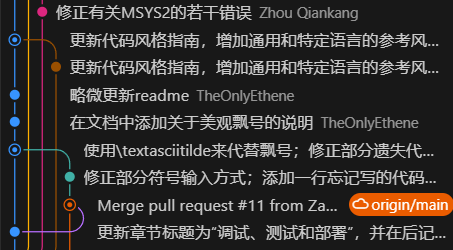
\includegraphics[width=0.8\textwidth]{images/git.png}
  \caption{一个典型的Git工作流程}
  \label{fig:git-workflow}
\end{figure}

\subsection{Git的工作原理}

Git有三个目录共同完成版本控制:工作区、暂存区、版本库。工作区是项目目录,暂存区是一个隐藏的文件夹.git,版本库是一个隐藏的文件夹.git/objects。工作区是我们平时使用的目录,暂存区是Git用来存储修改的地方,版本库是Git用来存储所有版本信息的地方。版本库有一个指针,指向当前版本的某一节点(一般指向最新的节点)。每个节点都有一个唯一的哈希值\footnote{哈希(Hash,也叫散列)指的是固定长度、像指纹一样的唯一小串字符,可用于快速校验、查找或加密等功能。},用来标识该节点。每个节点包含了该版本的所有文件和目录的信息,以及指向上一个版本的指针。Git使用哈希值来标识每个版本,这样可以保证每个版本都是唯一的。

这样讲解很难以理解,我们不妨举例说明:现在,Git中有一个版本为X的节点,包括文件A和文件B两个文件。这些文件存储在版本库中。此时,工作区为空,暂存区为空,指针指向X。我现在希望对它们进行修改,这个修改遵循以下过程:

\begin{enumerate}
  \item 我拿出了这些文件,并且对文件A进行修改。此时,工作区有AB两个文件,但是暂存区依然是空的。我们的任何修改都不会被暂存区记录,Git也不会知道我对这些文件进行了修改。

  \item 我觉得修改差不多了,现在把A放进暂存区。现在Git知道我对A进行了一些修改了。
    \begin{figure}[!ht]
      \begin{subfigure}[t]{0.45\linewidth}
        \centering
        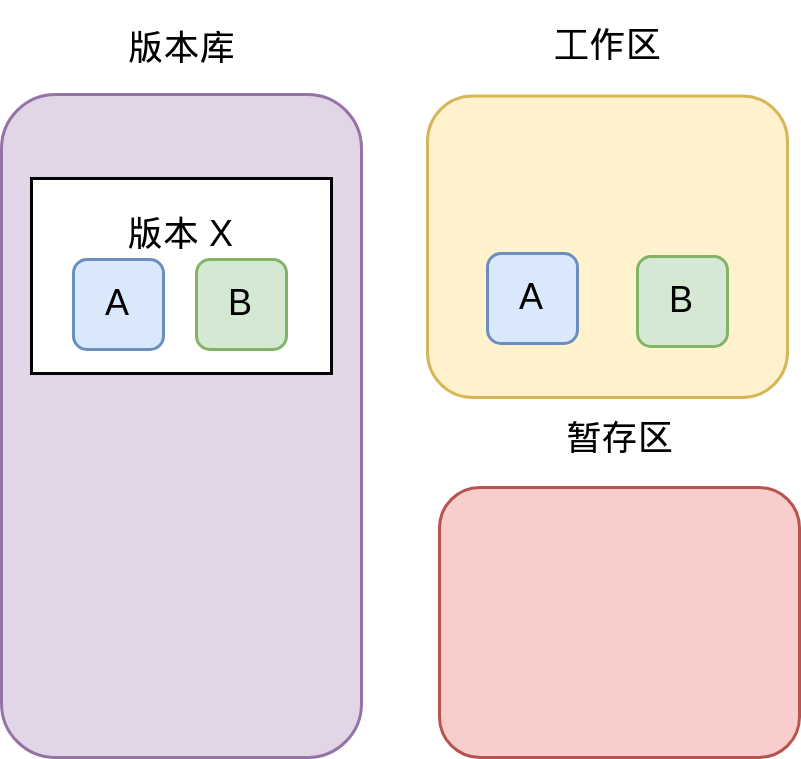
\includegraphics[width=\linewidth]{images/git-graph-no-modified.png}
      \end{subfigure}
      \hfill               % 把左右撑开
      %----- 右图 -----
      \begin{subfigure}[t]{0.45\linewidth}
        \centering
        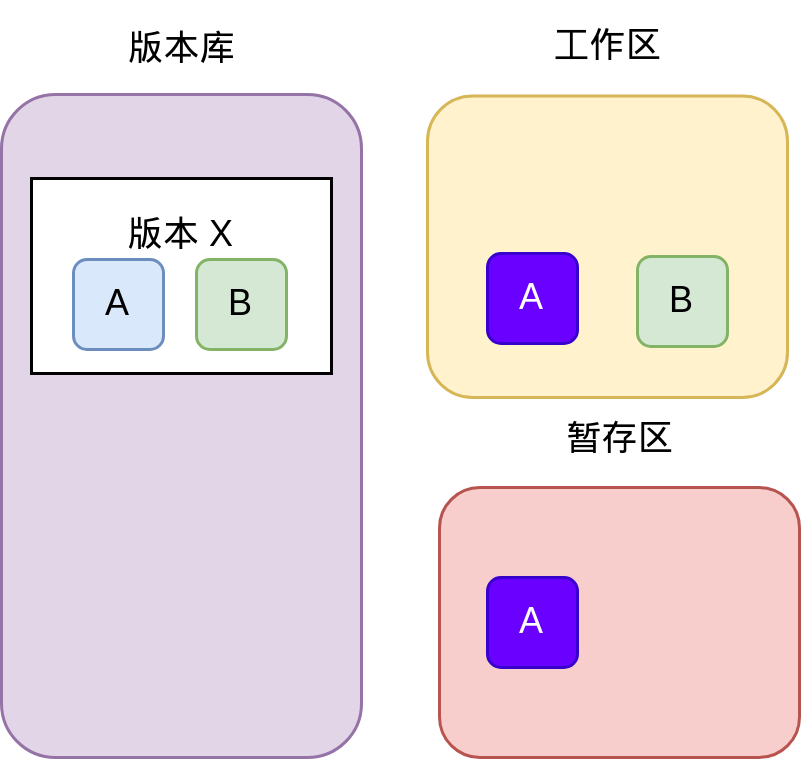
\includegraphics[width=\linewidth]{images/git-a-changed.png}
      \end{subfigure}
    \end{figure}
  \item 我又对B进行了类似的修改,此时B也进暂存区了。
  \item 我觉得修改差不多了。我认为我应该永久保存目前的状态,于是就把暂存区提交到版本库。此时版本库多了一个Y节点,指针也指向Y节点,有修改过的AB两个文件。此时,暂存区又清空了,而工作区和版本库的Y版本一致。
    \begin{figure}[!ht]
      \begin{subfigure}[t]{0.45\linewidth}
        \centering
        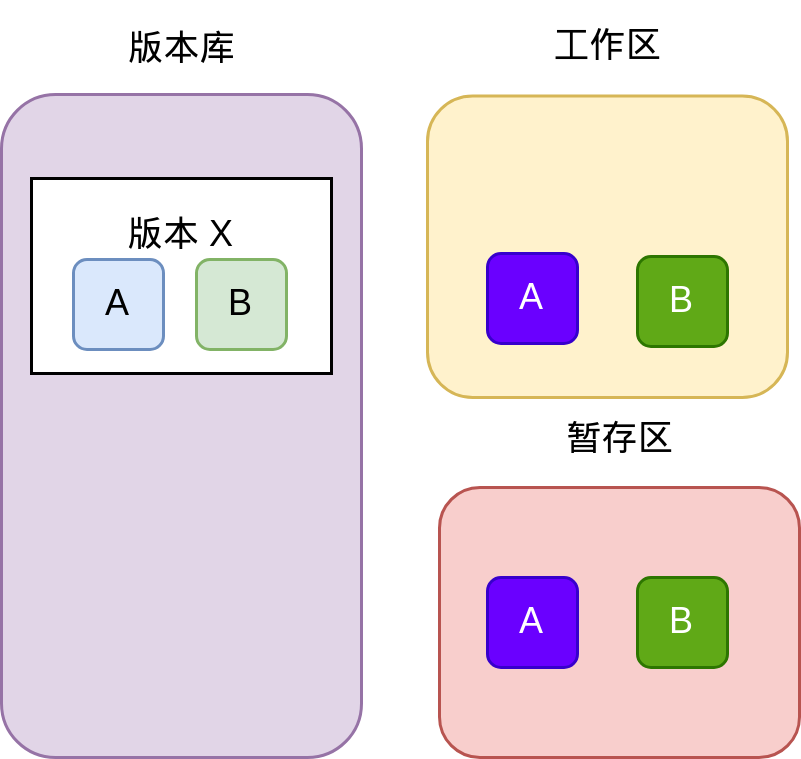
\includegraphics[width=\linewidth]{images/git-b-changed.png}
      \end{subfigure}
      \hfill               % 把左右撑开
      %----- 右图 -----
      \begin{subfigure}[t]{0.45\linewidth}
        \centering
        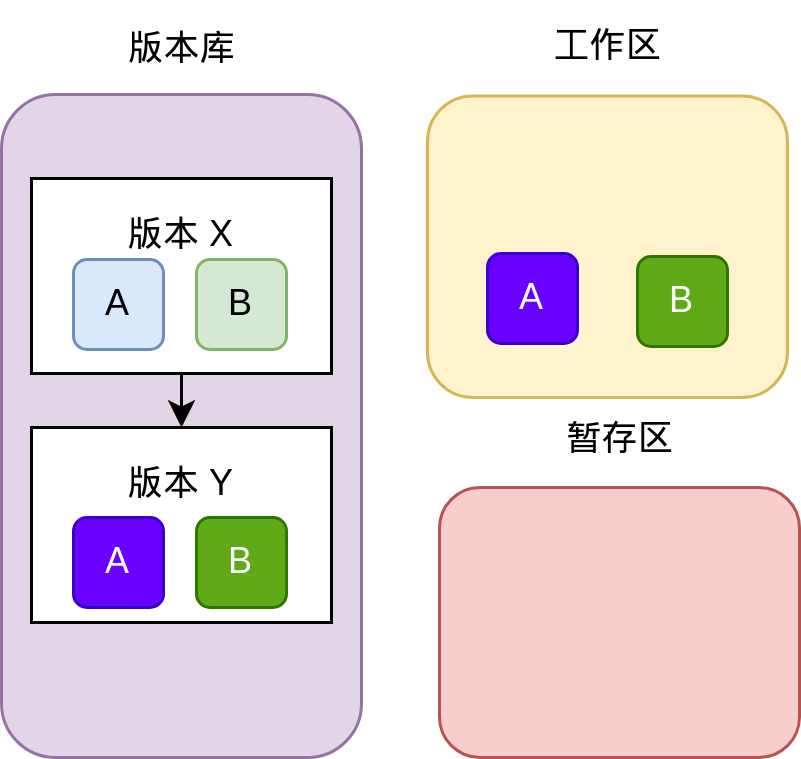
\includegraphics[width=\linewidth]{images/git-commited.png}
      \end{subfigure}
    \end{figure}
\end{enumerate}

\subsection{下载Git}

一个最简单的方式是使用Winget包管理器:

\begin{lstlisting}[language=bash]
    winget install Microsoft.git
\end{lstlisting}

或者你也可以从官方网站上下载并安装之。同样,安装的时候一定要勾选“添加到PATH”这一选项,否则你在命令行中无法使用Git。

\subsection{Git信息设置}

安装并使用Git的第一步是先编辑本地的一些信息。Git的提交需要一个用户名和一个邮箱,来对应每次提交的作者。我们可以使用以下命令来设置这些信息:

\begin{lstlisting}[language=bash]
    git config --global user.name "Your Name"
    git config --global user.email "email@example.com"
\end{lstlisting}

这样即可设置全局用户名和邮箱。如希望给某个特定仓库设置特定的用户名和邮箱,你需要在该仓库下重新执行上述命令,但是不写--global命令。

现代Git一般提倡使用main作为根分支的名称。而Git依然使用旧的master分支作为根分支,你可以使用以下命令修改为main:

\begin{lstlisting}[language=bash]
    git config --global init.defaultBranch main
    # 这条命令会修改全局的默认分支名称
\end{lstlisting}

\subsection{Git的最基本使用}

\subsubsection{提交}

要具体地在某一目录下进行版本控制,我们需要在命令行中进入到我们希望使用Git的目录下。然后我们可以使用以下命令来初始化一个Git仓库:

\begin{lstlisting}[language=bash]
    git init
\end{lstlisting}

如果你在视窗中开启了“显示隐藏文件”这类功能,你就会发现一个隐藏的文件夹.git出现在了你当前的目录下。这个文件夹就是Git用来存储版本信息的地方。

然后你可以使用以下命令来添加文件到Git仓库中(这个命令的实际意义是把文件添加到暂存区);

\begin{lstlisting}[language=bash]
    git add <filename>
\end{lstlisting}

如果我们忘记了当前状态下有哪些文件被修改了,我们可以使用以下命令来查看当前状态:
\begin{lstlisting}[language=bash]
    git status
\end{lstlisting}

如果你觉得修改差不多了,保存文件以后,你可以使用以下命令来提交文件到Git仓库中(这个命令的实际意义是把暂存区的文件提交到版本库中):

\begin{lstlisting}[language=bash]
    git commit -m "commit message"
\end{lstlisting}

上述内容中,-m后面是提交信息。提交信息是对本次提交的简要描述。我们建议每次提交都写上简要的提交信息,这样可以帮助我们更好地理解代码的修改历史。

\subsubsection{回退}

如果出现了先前我们说的不小心写坏了的情况,这时候就可以进行版本回退了。我们可以使用以下命令来查看当前的版本信息:

\begin{lstlisting}[language=bash]
    git log # 例如版本库是a-b-c-d-e-f-g
\end{lstlisting}

找到你希望回退到的版本的哈希值(前几位即可),然后使用以下命令来回退到该版本(这个命令会把指针回退到指定的版本,丢弃之后的所有内容,然后丢弃暂存区和工作区的所有东西):

\begin{lstlisting}[language=bash]
    git reset --hard <commit_hash>
    # 请谨慎使用这一命令!该命令不会保留当前的修改!
\end{lstlisting}

如果你希望回退到某个版本,但是不想丢失当前的修改,你可以使用以下命令来回退到该版本(这个命令会把版本库后面的东西全部丢弃,清空暂存区,但是保留当前工作区):
\begin{lstlisting}[language=bash]
    git reset --mixed <commit_hash>
    # 我们更加推荐这个回退方式,--mixed可以省略,或者用--soft替代。
    # 用--soft替代时,不会清空暂存区。
\end{lstlisting}

使用图解来表示一下:
\begin{figure}[htbp]
  \centering
  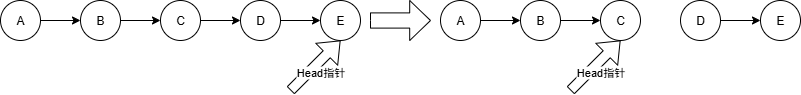
\includegraphics[width=0.8\textwidth]{images/git-reset.png}
  \caption{Git的回退操作}
  \label{fig:git-reset}
\end{figure}
可以看到,回退操作虽然会把指针回退到指定的版本并丢弃之后的版本,但是之后的版本提交依然存在于版本库中,只是被从树上摘下来了。这些提交被称为“孤立提交”。如果希望恢复或者删除这些孤立提交,可以执行以下命令:
\begin{lstlisting}[language=bash]
    git fsck --lost-found # 查看孤立提交、孤立分支等
    git checkout <commit_hash> # 进入分离头模式
    git branch <branch_name> # 创建一个分支来恢复孤立提交

    git gc --prune=now # 清理孤立提交
\end{lstlisting}
即使我们不使用\texttt{git gc}手动清理孤立提交,随着时间的推移(一般是90天提交记录过期),孤立提交也会被Git逐渐自动清理掉。

\subsubsection{排除相关文件}

有时候我们版本跟踪的时候不需要跟踪一些文件,例如具有敏感信息的文件(如密码),或者构建文件等。此时,我们可以创建一个文件 .gitignore 来阻止跟踪。例如,在Linux下,构建文件往往是*.o。那么我们可以在上述文件中加入 *.o ,之后git就会忽略这些文件。

关于Git版本控制的一些更加进阶的知识(例如分支管理等内容),欢迎查阅更多资料。我们在高阶课程\ref{sec:git-advanced}中会介绍一些Git的进阶用法。

\end{document}